\graphicspath{{img/ch3}}

\section{Thermal Characteristics}

\subsection{Thermal Stability and Anomalies}

The thermal environment within lunar pits provides a stark contrast to the extreme temperature fluctuations of the lunar surface. Data collected from the Diviner Lunar Radiometer Experiment reveal that the interior of pits maintains remarkably stable temperatures, ranging from 250 to 290 K in permanently shadowed regions, even during the lunar night \cite{thermal-lunar-pits}. This contrasts with the lunar surface, where temperatures vary dramatically between $\sim$100 K at night and $\sim$400 K in direct sunlight due to the Moon’s lack of atmosphere \cite{newer-thermal}.

\begin{figure}[H]
    \centering
    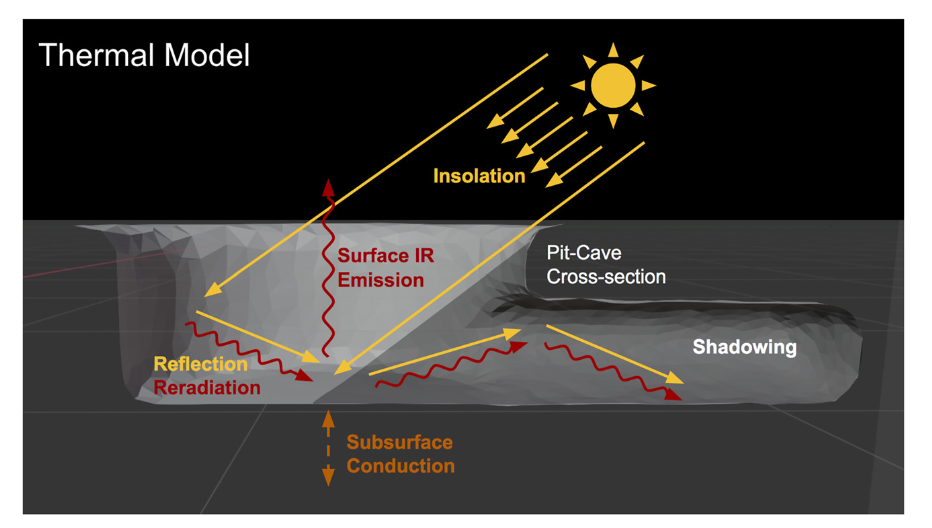
\includegraphics[width=0.6\linewidth]{lunar-pit-thermal-model.png}
    \caption{Schematic representation of heat transfer in lunar pits, illustrating shadowing, infrared emission, and subsurface conduction \cite{thermal-lunar-pits, newer-thermal}.}
    \label{fig:lunar-pit-thermal-model}
\end{figure}

The thermal stability results from the geometry of the pits, with overhanging walls and limited sky exposure blocking direct solar radiation and mitigating radiative heat loss during the lunar night. This configuration creates natural “blackbody cavities,” as modeled by Horvath et al. \cite{thermal-lunar-pits}, leading to effective absorption and internal redistribution of heat. For instance, pits such as those in Mare Tranquillitatis and Mare Ingenii have floors that remain up to 100 K warmer than their surroundings at night \cite{thermal-lunar-pits, newer-thermal, nesnas2019}.

The location of lunar pits relative to the equator or poles significantly impacts their thermal behavior. Pits closer to the equator, such as those in Mare Tranquillitatis, experience more extreme daytime temperature peaks due to higher levels of direct sunlight. In contrast, pits located closer to the poles maintain more stable temperatures, making thermal management less challenging. However, polar pits receive less sunlight, which reduces the availability of solar energy for power generation and may require hybrid energy systems to support exploration missions \cite{thermal-lunar-pits, newer-thermal}.

\begin{figure}[H]
    \centering
    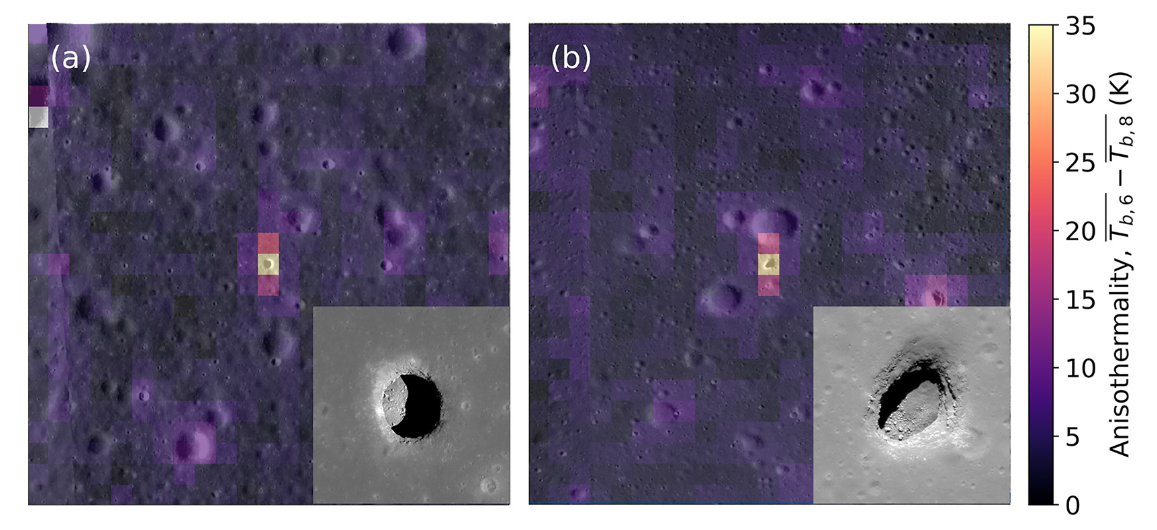
\includegraphics[width=0.7\linewidth]{lunar-pits-temperature-LROC.png}
    \caption{Temperature maps of Mare Tranquillitatis (a) and Mare Ingenii pits (b) measured by Diviner. Insets show NAC images for reference. Warm anomalies appear in pit interiors compared to surrounding surfaces \cite{thermal-lunar-pits}.}
    \label{fig:lunar-pits-temperatures-LROC}
\end{figure}

\subsection{Thermal Dynamics and Material Effects}

The thermal behavior of pit floors and walls depends strongly on their material composition. Regolith-dominated floors exhibit higher diurnal temperature variations due to their insulating properties, leading to pronounced daytime peaks and nighttime minima. In contrast, rock-dominated surfaces show smaller variations, as their higher thermal conductivity allows for more efficient heat transfer and equilibrium \cite{thermal-lunar-pits, newer-thermal}.

\begin{figure}[H]
    \centering
    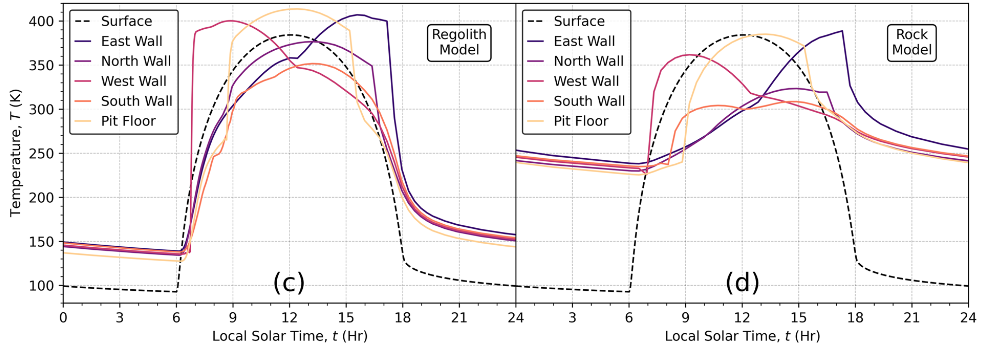
\includegraphics[width=0.9\linewidth]{lunar-pit-regolith-vs-stone-thermal.png}
    \caption{Simulated temperature profiles for lunar pits assuming regolith (c) and solid rock (d) floors. Rock surfaces show smaller diurnal variations due to higher thermal conductivity, while regolith exhibits greater fluctuations \cite{thermal-lunar-pits}.}
    \label{fig:regolith-vs-stone-thermal}
\end{figure}

The thermal behavior of lunar pits is strongly influenced by the nature of their floors. Pits with rocky floors maintain temperatures closer to equilibrium, as rock surfaces efficiently distribute absorbed heat, making them attractive for potential habitation and exploration. In contrast, regolith-covered floors retain heat near their openings and exhibit extreme thermal gradients. These gradients, resulting from the low thermal conductivity of lunar regolith, pose challenges for thermal management, especially during extended missions \cite{thermal-lunar-pits, newer-thermal}.

Numerical simulations show that rocky pit walls experience lower peak daytime temperatures and more gradual temperature variations compared to regolith surfaces, which insulate heat and cause significant temperature extremes. These properties highlight the need for tailored exploration strategies depending on the pit's material composition \cite{thermal-lunar-pits, lunar-pits-numerical-modelling}.

\begin{figure}[H]
    \centering
    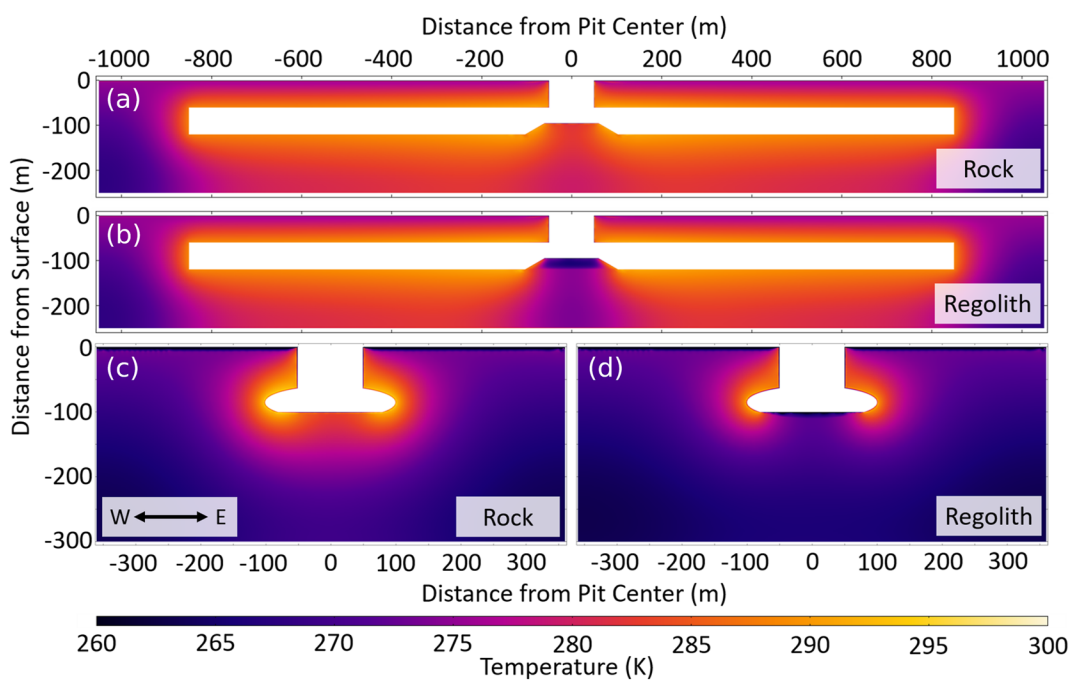
\includegraphics[width=0.8\linewidth]{thermal-simulation-lunar-pits-2d-regolith-rock.png}
    \caption{Equilibrium temperature distributions for rock (a, c) and regolith (b, d) surfaces in lunar pits and caves. Rock surfaces exhibit cooler and more uniform internal temperatures due to higher thermal conductivity, while regolith retains heat closer to the opening, leading to pronounced thermal gradients. Adapted from \cite{thermal-lunar-pits}.}
    \label{fig:lunar-pit-equilibrium-temps}
\end{figure}

\subsection{Volatile Stability and Cold Traps}

While lunar pits have been proposed as potential cold traps for volatiles like water ice, recent studies show that their enclosed geometry raises internal temperatures through multiple-scattered infrared radiation (see Fig. \ref{fig:lunar-pit-thermal-model}). This reduces their efficiency compared to traditional craters \cite{newer-thermal}. Nevertheless, specific conditions—such as pits shadowed by exterior topography or connected to deeper caves—could still support volatile accumulation \cite{thermal-lunar-pits, lunar-pits-numerical-modelling}.

Latitude affects volatile retention within pits. Pits closer to the poles experience lower maximum temperatures and are less likely to lose volatiles to sublimation compared to equatorial pits. However, the geometry of polar pits can still lead to elevated internal temperatures compared to permanently shadowed regions (PSRs), limiting their efficiency as long-term volatile storage sites \cite{newer-thermal, lunar-pits-numerical-modelling}.

Wilcoski et al. \cite{newer-thermal} demonstrate that while volatile loss rates in pits are higher than in PSRs, certain configurations—such as pits with deeper caves or extended shadowed regions—may still allow for temporary volatile preservation. These findings suggest that lunar pits could serve as short-term repositories for accessible volatiles during exploration missions.
